%\documentclass[11pt]{scrartcl}

%ronny
\documentclass[12pt]{scrreprt}

\usepackage{primaer}
\usepackage{setspace}
\usepackage{txfonts}
\usepackage{algorithm}
\usepackage[ngerman]{babel}
%\usepackage{algorithm}
\usepackage{algorithmic}
\usepackage{tikz}
\usetikzlibrary{trees}
\usetikzlibrary{shapes}
\usetikzlibrary{automata}
\usetikzlibrary{backgrounds}
\usetikzlibrary{plotmarks}
\usetikzlibrary{arrows}
%ende ronny

%\geometry{a4paper,left=25mm,right=50mm, top=13mm, bottom=20mm}
%\geometry{a4paper,right=50mm,left=25mm}
\newcommand{\ff}{\triangleright}
\newcommand{\pref}[1]{\mathit{pref{#1}}}
\renewcommand{\min}{\mathit{Min}\;}

\newtheorem{def1}{Definition}
\newtheorem{satz}{Satz}
\newtheorem{lem}{Lemma}
\newtheorem{bew}{Beweis} 
\newtheorem{gleich}{Gleichung}[section]
\newtheorem{eigen}{Eigenschaft}
\newtheorem{folg}{Folgerung}
\theoremstyle{remark}
\newtheorem{beispiel}{Beispiel}

\author{Robert Hartmann}
\title{"Uber die Operation Fortsetzung bei formalen Sprachen}
\date{24. September 2010}
\parindent 0pt
\begin{document}

\pagestyle{empty}

\begin{center}

{\Large\sc Bachelorarbeit}

\vspace{1.25cm}

{\fontsize{22}{22}\selectfont "Uber die Operation Fortsetzung\\bei formalen Sprachen}

\vspace{1.25cm}

{\Large\sc

Robert Hartmann

\vspace{.15cm}

Betreuer: Prof. Dr. Ludwig Staiger

\vspace{.15cm}

24. September 2010

}

\vspace{10.5cm}

\begin{tabular}{c}
	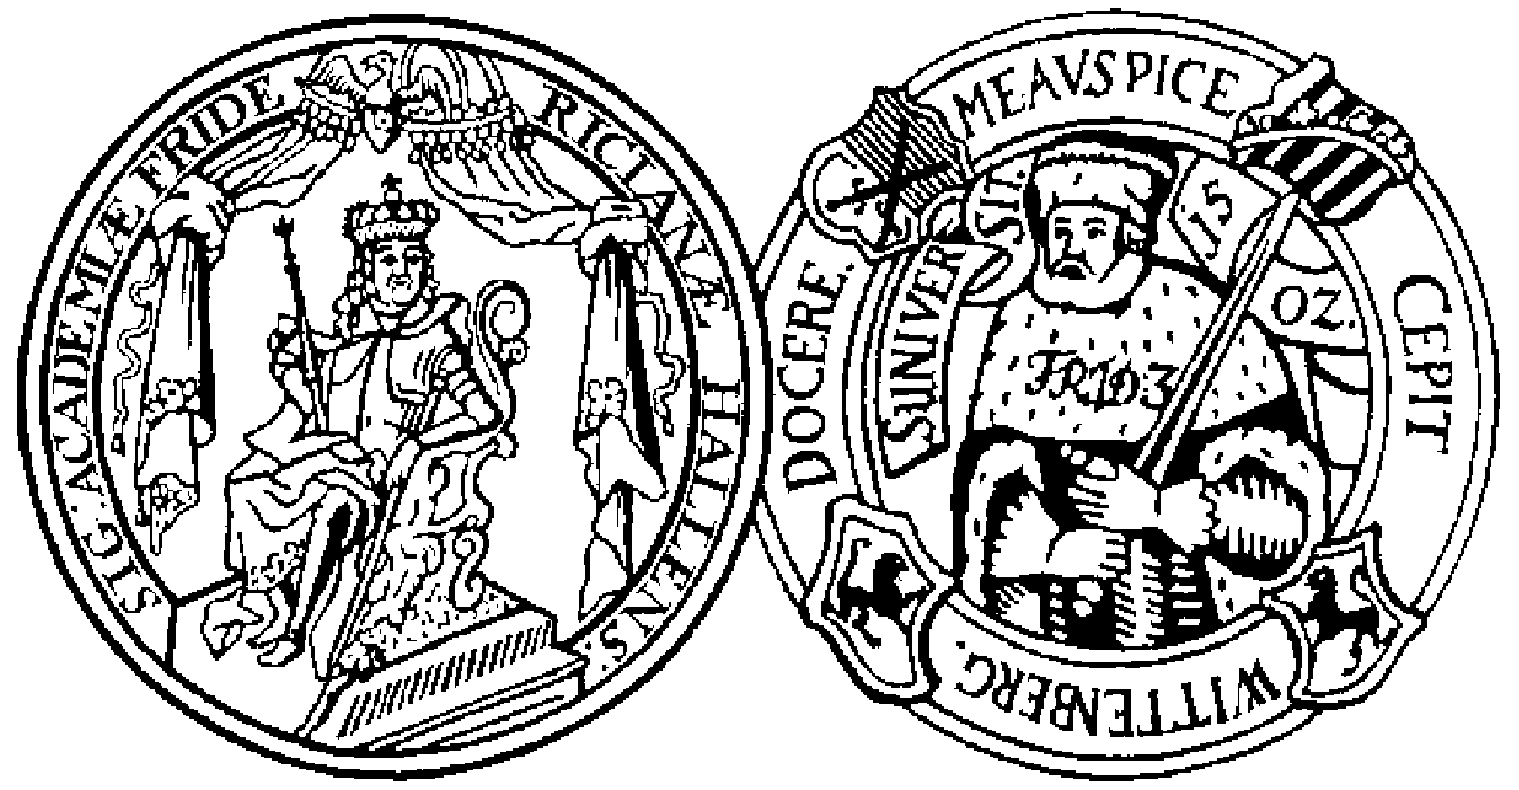
\includegraphics[height=15ex]{Bilder/siegel}
\end{tabular}

\vspace{0.5cm}

\rule{.7\textwidth}{.40pt}

\vspace{.2cm}

{\large\sc

martin-luther-universit"at halle-wittenberg

}

\end{center}

\cleardoublepage


%\include{dedication}

\pagestyle{plain}
\tableofcontents[hideallsubsections]

\onehalfspacing

\chapter{Einleitung}
%einleitung
In dieser Arbeit wird die Operation Fortsetzung bei formalen Sprachen untersucht.
Im Folgenden wird erl�utert warum die Operation in [St87] eingef�hrt wurde und welchen Nutzen sie birgt.\\\\
Wir bezeichnen die Menge $X^*$ als Menge aller endlichen W�rter �ber dem Alphabet $X$. 
\\Wir bezeichnen weiterhin die Menge $X^\omega$ als Menge aller unendlichen W�rter �ber dem Alphabet $X$.
\\Sei ferner die Relation $\sqsubseteq$ wie �blicherweise definiert:
\begin{def1}
$$w\sqsubseteq b \Leftrightarrow w\cdot b' = b,\textit{ f{\"u}r ein }b'\in X^*$$
$$\pref(L) = \{v:v\sqsubseteq w \wedge w\in L\}$$
\end{def1}
Sei nun $W ^\delta$ definiert \footnote{St87]}
\begin{def1}
$$W^\delta = \{\beta : \beta \in X^\omega \textit{ und }\pref(\beta)\cap W \textit{ ist unendlich}\}$$
\end{def1}
% also eine unendliche Aneinanderreihung von W�rtern aus ....
Folgende Eigenschaft wurde nun bereits in \footnote{[St87, Gleichung 13]} bewiesen:
$$(U \cup W)^\delta = U^\delta \cup W^\delta $$
	\begin{def1}
	Eine Sprache nennen wir eine $(\sigma,\delta)$-Teilmenge von $X^*$ genau dann, wenn f�r alle $\beta \in X^\omega$ entweder $\pref(\beta)\cap W$ oder $\pref(\beta)\backslash W$ endlich ist.	
	\end{def1}
Beispiele f�r $(\sigma,\delta)$-Teilmengen sind alle endlichen Sprachen und deren Komplemente. Weitere Beispiele sind Sprachen der Form $\pref(U)$ oder $W\cdot X^*$.\\
Eine Eigenschaft f�r diese Teilmengen lautet wiefolgt:
\begin{satz}
$\text{Sei }U\text{ eine }(\sigma,\delta)-\text{Teilmenge von }X^*, \text{ dann gilt:}$\\
$$(U\cap W)^\delta = U^\delta \cap W^\delta,\qquad \text{f�r alle }W\subseteq X^*$$
\end{satz}

Nun wird die Operation "'Fortsetzung"' eingef�hrt \footnote{[St87, S.170]}, im nachfolgenden als $\ff$ bezeichnet.
Die Fortsetzung eines Wortes $w$ in $V$ sei definiert als:
\begin{def1}
$$w\ff V := \min_{\sqsubseteq} \{v:v\in V \wedge w\sqsubseteq v\} = \min(w\cdot X^* \cap V)$$
\end{def1}
Man kann diese Definition nun ausdehnen auf Sprachen. Die Fortsetzung zweier Sprachen W und V ergibt sich somit zu:
\begin{def1}
$$W\ff V := \bigcup_{w\in W} w\ff V$$
\end{def1}
Diese Operation hat nun folgende interessante Eigenschaft bez�glich der oben genannten Definitionen:
W�hrend $$(W\cap U)^\delta = W^\delta \cap U^\delta$$ nur f�r $(\sigma,\delta)$-Teilemgen gilt, so gilt aber
$$(W\ff U)^\delta = W^\delta \cap U^\delta$$ f�r s�mtliche Sprachen \footnote{[St87, Gleichung 20]}\\
Daher wird nun im Verlauf der Arbeit die Operation Fortsetzung gr�ndlich analysiert und all ihre Eigenschaften dokumentiert.


\chapter{Notation}
%notationen
Mit $\mathbb{N}=\{0,1,2,3,..\}$ bezeichnen wir die Menge der nat�rlichen Zahlen. Es sei $X$ ein Alphabet.
Mit $X^*$ bezeichnen wir die Menge aller endlichen W�rter �ber dem Alphabet $X$, einschlie�lich des leeren Wortes $e$.
Wir bezeichnen weiterhin die Menge $X^\omega$ als Menge aller unendlichen W�rter �ber dem Alphabet $X$.\\\\
F�r $w\in X^*$ und $v\in X^* \cup X^\omega$ bezeichne $w\cdot v$ die Konkatenation von $w$ und $v$. Daraus ergibt sich in nat�rlicher Weise ein Produkt $L\cdot W$ von Mengen $L\subseteq X^*$ und $W\subseteq X^*\cup X^\omega$.
F�r eine Sprache $W$ ist $W^*=\bigcup_{i\in\mathbb{N}} W^i$. Weiterhin bezeichne $\vert w\vert$ die L�nge des Wortes $w\in X^*$.
Wir definieren die Pr�fixrelation $\sqsubseteq$ wie �blich mit $w\sqsubseteq b \Leftrightarrow w\cdot b' = b,\textit{ f{\"u}r ein }b'\in X^*$.
Somit bildet $\pref(L) = \{v:v\sqsubseteq w \wedge w\in L\}$ alle Pr�fixe aller W�rter aus $L$.\\\\
Weiterhin bezeichnen wir mit $\min(L) = \{w:w\in L \wedge \forall v( v\sqsubset w \to v\notin L)\}$ alle W�rter der Sprache $L$, in denen kein Wort Pr�fix eines anderen Wortes ist.
Die Fortsetzung $\ff$ eines Wortes $w$ in $L$ definieren wir als $w\ff L = \min(w\cdot X^* \cap L)$. Diese Definition weiten wir auf Sprachen aus und definieren
die Fortsetzung einer Sprache $L$ in die Sprache $W$ als $L\ff W = \bigcup_{u\in L} u\ff W$\\\\
Wir definieren den $\delta$-Limes einer Wortmenge $W ^\delta$ wie in [St87] mit\\$W^\delta = \{\beta : \beta \in X^\omega \text{ und }\pref(\beta)\cap W \text{ ist unendlich}\}$
% also eine unendliche Aneinanderreihung von W�rtern aus ....
Die Eigenschaft (13) aus [St87] ist leicht einzusehen: $(U \cup W)^\delta = U^\delta \cup W^\delta$.	Eine Sprache nennen wir eine $(\sigma,\delta)$-Teilmenge von $X^*$ genau dann, wenn f�r alle $\beta \in X^\omega$ entweder $\pref(\beta)\cap W$ oder $\pref(\beta)\setminus W$ endlich ist.
Beispiele f�r $(\sigma,\delta)$-Teilmengen sind alle endlichen Sprachen und deren Komplemente. Weitere Beispiele sind Sprachen der Form $\pref(L)$ oder $W\cdot X^*$.\\
F�r den Durchschnitt gilt nur $(U\cap W)^\delta = U^\delta \cap W^\delta$, falls einer der beiden Operanden eine $(\sigma,\delta)$-Teilmenge ist.
Die Operation der Fortsetzung $\ff$ wurde in [St87] eingefuehrt, um den Durchschnitt zweier $\delta$-Limites zu beschreiben.


\chapter{Eigenschaften}
\subsection{Gilt f�r alle Sprachen}

Folgende Eigenschaft ist direkt aus der Definition einsehbar:
\begin{gleich}
$$u\in L \to (u\ff L=\{u\})$$
\end{gleich}

Aus 2.1.1 folgt direkt
\begin{gleich}
$$L\ff L = L$$
\end{gleich}
\begin{gleich}
$$U\ff L \subseteq L$$
\end{gleich}

Eine unmittelbare Folgerung aus der Definition 1.5 ergibt sich:
\begin{gleich}
$$(L\cup U)\ff V = (L\ff V) \cup (U\ff V)$$
\end{gleich}
\begin{proof}
$$(L\cup U) \ff V = \bigcup_{l\in L\cup U} \min(l\cdot X^* \cap V)$$
$$ =\bigcup_{l\in L} \min(l\cdot X^* \cap V) \cup \bigcup_{l\in U} \min(l\cdot X^* \cap V)$$
$$ = (L\ff V) \cup (U\ff V)$$
\end{proof}

Aus dieser Gleichung 2.1.4 folgt wiederum direkt:

\begin{gleich}
$$L_2\subseteq L_1 \to L_2\ff W \subseteq L_1 \ff W$$
\end{gleich}
\begin{proof}
$$L_1\ff W = \bigcup_{l\in L_1} l\ff W$$
$$=\bigcup_{l\in L_2} l\ff W \cup \bigcup_{l\in L_1\backslash L_2} l\ff W$$
$$\supseteq \bigcup_{l\in L_2} l\ff W = L_2\ff W$$
\end{proof}

Auf Gleichung 2.1.5 folgt direkt:

\begin{gleich}
$$(L\cap U) \ff V \subseteq (L\ff V) \cap (U\ff V)$$
\end{gleich}
\begin{proof}
$$w\in  (L\cap U)\ff V \to w\in V \wedge \exists p: p\sqsubseteq w \wedge p\in L \wedge p\in U \wedge p\textit{ ist minimal}$$
$$\to \underbrace{w\in V \wedge \exists p: p\sqsubseteq w \wedge p\in L \wedge p\textit{ ist minimal}}_{w\in L\ff V} 
\wedge \underbrace{w\in V \wedge \exists p: p\sqsubseteq w \wedge p\in U \wedge p\textit{ ist minimal}}_{w\in U\ff V} 
$$
\end{proof}


\begin{gleich}
$$L\ff (U\cup V)\subseteq (L\ff U) \cup (L\ff V)$$
\end{gleich}
\begin{lem}
$$\min (A\cup B) \subseteq \min A \cup \min B$$
\end{lem}
Es gen�gt, die Eigenschaft f�r $L=\{w\}$ zu zeigen.
\begin{proof}
$$L\ff (W\cup V)= w \ff (W\cup V)$$
$$=\min (w\cdot X^* \cap (W\cup V))$$
Nach Anwenden der Distributivgesetze ergibt sicht:
$$=\min ((w\cdot X^* \cap W) \cup (w\cdot X^* \cap V))$$
Anwendung von Lemma 1:
$$\subseteq \min (w\cdot X^* \cap W) \cup \min (w\cdot X^* \cap V)$$
$$=(L\ff W)\cup (L\ff V)$$
\end{proof}

\begin{gleich}
$$L\ff (U\cap V)\supseteq (L\ff U) \cap (L\ff V)$$
\end{gleich}
\begin{lem}
$$\min(A\cap B) \supseteq \min A \cap \min B$$
\end{lem}
Es gen�gt die Eigenschaft f�r $L=\{w\}$ zu zeigen.
%\begin{lem}
%$$L\ff U \cap L \ff V \stackrel{!}{=} \bigcup_{l\in L} (l\ff U \cap l\ff V)$$
%\end{lem}
\begin{proof}
$$L\ff (U\cap V) = \min(w\cdot X^* \cap (U \cap V))$$
Nach Anwenden der Distributivgesetze ergibt sicht:
$$= \min((w\cdot X^* \cap U) \cap (w\cdot X^* \cap V))$$
Anwendung von Lemma 2:
$$\supseteq \min(w\cdot X^* \cap U) \cap \min(w\cdot X^* \cap V)$$
$$=(L\ff U) \cap (L\ff V)$$
\end{proof}

\begin{gleich}
$$L_1\subseteq L_2 \to L_1\ff L_2 = L_1$$
\end{gleich}
\begin{eigen}
$$l\in L \to l\ff L = \{l\}$$
\end{eigen}
\begin{proof}
$$L_1\ff L_2 = \bigcup_{l\in L_1} l\ff L_2$$
$$\textit{wegen } L_1\subseteq L_2: l\ff L_2 = \{l\}$$
$$ = \bigcup_{l\in L_1} \{l\} = L_1$$
\end{proof}

\begin{gleich}
$$L_2\subseteq L_1 \to L_1\ff L_2 = L_2$$
\end{gleich}
\begin{proof}
$$\textit{Da }L_2\subseteq L_1\textit{ gilt f�r alle }l\in L_2 \wedge l\in L_1: l\ff L_2=\{l\}$$
$$\bigcup_{l\in L_1} l\ff L_2 = \bigcup_{l\in L_1} \{l\} = L_2$$
\end{proof}

\subsection{Gilt f�r einige Sprachen $\exists L,U,V \subseteq X^*:$}
$$L\ff (U\cdot V) = (L\ff U) \cdot (L\ff V)$$
$$L\ff (U\cdot V) \supset (L\ff U) \cdot (L\ff V)$$


\subsection{Gilt nicht...}
Folgt direkt aus den Gleichungen in 2.1
$$L\ff (U\cup V)\supset (L\ff U) \cup (L\ff V)$$
$$L\ff (U\cap V)\subset (L\ff U) \cap (L\ff V)$$
$$L\ff (U\cdot V)\subset (L\ff U) \cdot (L\ff V)$$
$$(L\cap U) \ff V \supset (L\ff V) \cap (U\ff V)$$

\newpage
$$L\ff (U\cup V)\subset (L\ff U) \cup (L\ff V)$$
$$L= \{a,b\} U =\{aaa\} V = \{bb,aa\}$$\\
$$L\ff (U\cup V) = (L\ff U) \cup (L\ff V)$$
$$L= \{a,b\} U =\{aaa\} V = \{aaa\}$$\\
$$L\ff (U\cap V)\supset (L\ff U) \cap (L\ff V)$$
$$L= \{a,b\} U =\{aaa,b,bb\} V = \{bb,aaa\}$$\\
$$L\ff (U\cap V)= (L\ff U) \cap (L\ff V)$$
$$L= \{a\} U =\{aaa\} V = \{aaa\}$$\\
$$(L\cap U) \ff V \subset (L\ff V) \cap (U\ff V)$$
$$L= \{aa,bb\} U = \{aa,b\} V = \{aa,bb\}$$\\
$$(L\cap U) \ff V = (L\ff V) \cap (U\ff V)$$
$$L= \{aaa\} U =\{aaa\} V = \{aaa\}$$\\
\vspace{5mm}
$$L\ff (U\cup V) \not\supset (L\ff U) \cup (L\ff V),$$
$$\text{Gegenbeispiel: } L=\{a\}\quad U=\{abb,aaba\}\quad V=\{aab,aba\} $$
$$L\ff (U\cup V) = \{abb,aba,aab\}\text{ ,aber } L\ff U \cup L\ff V = \{abb,aaba\} \cup \{aab,aba\} = \{abb,aaba,aab,aba\} $$
\vspace{5mm}
$$L\ff (U\cap V) \not\subset (L\ff U) \cap (L\ff V),$$
$$\text{Gegenbeispiel: } L=\{a,b\}\quad U=\{a,aa\}\quad V=\{aa,b\} $$
$$L\ff (U\cap V) = \{aa\}\text{ ,aber } L\ff U \cap L\ff V =
\{a\} \cap \{b\} = \emptyset $$
\vspace{5mm}
$$L\ff (U\cdot V)= (L\ff U) \cdot (L\ff V),$$
$$\text{Beispiel: } L=\{e\}\quad U=\{a\}\quad V=\{b\} $$
$$L\ff (U\cdot V) \supset (L\ff U) \cdot (L\ff V),$$
$$\text{Beispiel: } L=\{a\}\quad U=\{aa\}\quad V=\{b,a\} $$
\vspace{5mm}
$$(L_1 \ff L_2) \ff L_3 \nsupseteq L_1 \ff (L_2 \ff L_3)$$
$$\text{Gegenbeispiel: } L_1=\{ab,aa\}\quad L_2=\{a,ab\}\quad L_3=\{aa\}$$
$$(L_1 \ff L_2) \ff L_3 = \{ab\} \ff \{aa\} = \emptyset\text{ ,aber } 
\{ab,aa\} \ff \{aa\} = \{aa\} $$


\chapter{Eigenschaften bei Sprachen spezieller Gestalt}
%\begin{eigen}
%$$V\ff W\cdot X^* = V\ff W $$
%\end{eigen}

%Es gen�gt die Eigenschaft zu zeigen f�r $L=\{v\}$:
%\begin{proof}
%$$V\ff W\cdot X^* = \{v\} \ff W\cdot X^*$$
%Nach Definition der Operation Fortsetzung ergibt sich:
%$$ = min_{\sqsubseteq} \{w:w\in W\cdot X^* \wedge v\sqsubseteq w\}$$
%Wir wissen aus der Vorrausetzung, dass $v\notin W\cdot X^*$, daraus folgt unmittelbar, dass $v\in pref(W)\backslash W$.\\
%Angenommen es existiert ein $w\in W\cdot X^+$ in $min_{\sqsubseteq} \{w:w\in W\cdot X^* \wedge v\sqsubseteq w\}$, so ist $w'$ mit $w=w'\cdot r\wedge w'\in W$ ein k�rzeres Wort, daher gilt:
%$$min_{\sqsubseteq} \{w:w\in W\cdot X^* \wedge v\sqsubseteq w\} = min_{\sqsubseteq} \{w:w\in W \wedge v\sqsubseteq w\}$$
%\end{proof}

%\begin{eigen}
%$$V\ff W = V\ff \min(W)$$
%\end{eigen}

\begin{lem}\label{eingeschr1}
Sei $V\subseteq X^*\backslash W\cdot X^*$, so gilt $V\ff W\cdot X^* = V\ff \min(W) $
\end{lem}
z.z:\\\\
1. $V\ff W\cdot X^* \subseteq V\ff \min(W) $\\
2. $V\ff W\cdot X^* \supseteq V\ff \min(W) $\\

\textbf{zu 1.} Es gen�gt die Eigenschaft zu zeigen f�r $V=\{v\}$\\
\begin{proof}
$$v \ff W\cdot X^* = \min_{\sqsubseteq} \{w:w\in W\cdot X^* \wedge v\sqsubseteq w\}$$
$$w\in W\cdot X^* \wedge v\sqsubseteq w \wedge v\not\in W\cdot X^* \to ( w'\in (\min(v\cdot X^* \cap W\cdot X^*) \to w'\in  (\min(v\cdot X^* \cap \min(W)))) )$$
\end{proof}

\textbf{zu 2.} klar, weil $W\cdot X^* \supseteq \min(W)$



\newpage

\begin{eigen}
$\pref(V)\ff W$
\end{eigen}
\begin{proof}
1. Fall: $w\in W \cap \pref(V) \to w\in \pref(V)\ff W$\\
2. Fall: $w\in W\backslash \pref(V) \to w\in V\ff Min(W)$\\
$\to \pref(V)\ff W = (\pref(V)\cap W) \cup (\pref(V)\ff \min(W))$\\\\
\end{proof}

\begin{eigen}
$W\ff \pref(V) = W \cap \pref(V)$
\end{eigen}
Es gen�gt die Eigenschaft f�r $W=\{w\}$ zu zeigen:
\begin{proof}
$$W\ff \pref(V) = \{w\}\ff\pref(V)$$
$$=min_{\sqsubseteq} \{v:v\in \pref(V) \wedge w\sqsubseteq v\}$$
Aus $v\in \pref(V) \wedge w\sqsubseteq v$ folgt direkt, dass $w\in pref(V)$. Damit ergibt sich :
$$min_{\sqsubseteq} \{v:v\in \pref(V) \wedge w\sqsubseteq v\} = \{v:v\in\pref(V)\wedge w=v\} = \{w\} \cap \pref(V)$$
\end{proof}
%"'$\leftarrow$"'\\
%$w\in \pref(V) \wedge w\in W \to w\sqsubseteq v\in \pref(V)$\\\\
\begin{eigen}
$V\cdot X^* \ff W$
\end{eigen}
Es gen�gt die Eigenschaft f�r ein $v\in V\cdot X^*$ zu zeigen:
\begin{proof}
$$\min_{\sqsubseteq} \{w:w\in W \wedge v\sqsubseteq w\}$$
$$v\in VX^* \wedge v\sqsubseteq w \to w\in VX^*$$
$$=\min_{\sqsubseteq} \{w:w\in W \wedge w\in V\cdot X^* \wedge v=w\} = \{v\}\cap W$$
%$=\bigcup_{v\in V} \{w:w\in W \wedge v\sqsubseteq w\}$\\\\
\end{proof}

\begin{eigen}
$$W\ff V\cdot X^*$$
\end{eigen}
\begin{proof}
$W$ l�sst sich in 2 Teile aufspliten: $W= (W\cap V\cdot X^*) \cup (W\backslash V\cdot X^*)$
Nun betrachten wir folgende 2 F�lle:\\\\
Fall a) $w\in W\cap V\cdot X^*$\\
Fall b) $w\in W\backslash V\cdot X^*$\\\\
zu a): $w\ff V\cdot X^* \to w\in (W\cap V\cdot X^*)$\\
zu b): Es gilt nach Vorraussetzung $\{w\} \subseteq X^*\backslash V\cdot X^*$ und mit Hilfe von Lemma~\ref{eingeschr1}
erhalten wir $\{w\} \ff V\cdot X^* = \{w\} \ff \min(V)$
\\Daraus folgt: $$W\ff V\cdot X^* = (W\ff\min(V)) \cup (W\cap V\cdot X^*)$$
\end{proof}





%\newpage
%$$ V = \{v:\forall w(w\in W \to w\not\sqsubseteq v)\}\qquad \mathit{pref}(V)=\{u:\exists v (u\sqsubseteq v\wedge v\in V)\}$$\\
%$$W\ff V = \emptyset$$
%$$W\ff \mathit{pref}(V) = \emptyset$$
%$$W\cdot X^* \ff V = \emptyset$$
%$$W\cdot X^* \ff \mathit{pref}(V) = \emptyset$$
%$$\mathit{pref}(V)\ff W\cdot X^* = $$

%$$W\ff V = \bigcup_{x\in W} x\ff V = \bigcup \min_{\sqsubseteq } \{v:v\in V \wedge x\sqsubseteq v\}$$
%Wegen $x\in W$ und $x\sqsubseteq v$ gilt $\{v:v\in V \wedge x\sqsubseteq v\} = \emptyset \Rightarrow \bigcup \min_{\sqsubseteq} \{v:v\in V \wedge x\sqsubseteq v\} = \emptyset$\\\\
%$$ W\cdot X^* \ff V = \bigcup_{x\in W\cdot X^*} x\ff V = \bigcup_{x\in W\cdot X^*} \min_{\sqsubseteq} \{v:v\in V \wedge x\sqsubseteq v\} = \emptyset$$
%Begr�ndung analog Fall $W\ff V$\\\\
%$$ W \ff \mathit{pref}(V) = \bigcup_{w\in W} w\ff \mathit{pref}(V) = \bigcup_{w\in W} \{v:v\in \mathit{pref}(V) \wedge w\sqsubseteq v\} = \emptyset$$
%$w\sqsubseteq v$ ist nie erfuellt. Angenommen $v\in \mathit{pref}(V) \wedge w\sqsubseteq v$, dann kann man $v$ wie folgt verlaengern $v'=v\cdot v''$ mit $v'\in V$, dann waere $v'=w\cdot w' \cdot v''$ mit $w\cdot w' = v$.
%Dadurch gilt aber $v'\in V\wedge w\sqsubseteq v' \wedge w\in W \Rightarrow$ Widerspruch zur Definition.\\\\

%$$\mathit{pref}(V) \ff W\cdot X^* = \bigcup_{u\in \mathit{pref}(V)} u\ff W\cdot X^* = \bigcup_{u\in \mathit{pref}(V)} \min_{\sqsubseteq} \{w:w\in W\cdot X^* \wedge u\sqsubseteq w\}$$
%$$ =  \bigcup_{u\in \mathit{pref}(V)} \min(W\cdot X^* \cap u\cdot X^*) =  \bigcup_{u\in \mathit{pref}(V)} \min(\{w:w\in W \wedge u\sqsubseteq w\})$$\\
%$$W\cdot X^* \ff \mathit{pref}(V) = \bigcup_{u\in W\cdot X^*} u\ff \mathit{pref}(V) = \bigcup_{u\in W\cdot X^*} \min_{\sqsubseteq} \{w:w\in \mathit{pref}(V) \wedge u\sqsubseteq w\}$$
%$$ = \bigcup_{u\in W\cdot X^*} \min(\mathit{pref}(V)\cap u\cdot X^*)$$
%$\mathit{pref}(V)\cap u\cdot X^* = \emptyset$, Begr�ndung siehe oben $\Rightarrow  \bigcup_{u\in W\cdot X^*} \min(\emptyset) = \emptyset$


\chapter{Abgeschlossenheitseigenschaften}
In diesem Abschnitt untersuchen wir die Abgeschlossenheitseigenschaften der Klassen der CHOMSKY-Hierachie bez"uglich der Operation Fortsetzung. 
Dabei betrachten wir in den folgenden Abschnitten die Klassen der regul"aren, kontextfreien, entscheidbaren und aufz"ahlbaren Sprachen.

\section{Regularit"at}\label{abschnittreg}
\begin{satz}
Sind $L$ und $W$ regul\"are Sprachen, so ist auch $L\ff W$ regul\"ar.
\end{satz}
\begin{proof}
Der nichtdeterministische Automat $A_L= (X,Z,z_{0},\delta_L,Z_f)$ akzeptiere $L$, der deterministische Automat $A_W = (X,S,s_{0},f,S_{f})$ akzeptiere $W$.
Wir konstruieren einen nichtdeterministischen Automaten $A$, der $L\ff W$ akzeptiert.\\\\\emph{Arbeitsweise.}\\
In Phase eins lesen $A_L$ und $A_W$ das Wort $w$ parallel (\ref{auto1}). Falls $A_L$ ein Pr"afix $v$ von $w$ akzeptiert, w"ahlt $A$ nichtdeterministisch aus, ob Schritt zwei aktiviert wird oder nicht ( Nichtdeterminismus von $A_L$ ).\\
Wird Phase zwei aktiviert, so liest $A_W$ das Wort $w$ weiter, w"ahrend $A_L$ in einem Ruhezustand $z_f'$ verweilt (\ref{auto2}). Sobald $A_W$ in Phase zwei akzeptiert, gelangt $A$ nach Konstruktion in den Zustand $(z_f',s_x)$, aus dem keine Transition herausf"uhrt (\ref{auto4}). Akzeptiert $A_W$ nun ein Pr"afix $v'$ mit $v\sqsubseteq v'\sqsubset w\text{ und } v'\in W$, so muss $A$ das Eingabewort $w$ ablehnen. Dies wird realisiert, da keine Transition aus $(z_f',s_x)$ herausf"uhrt und $w$ noch nicht zu Ende gelesen ist. Findet der Automat $A_W$ kein solches Pr"afix $v'$ und akzeptiert das Eingabewort $w$ ( und kein Pr"afix von $w$), so akzeptiert auch $A$, weil $w$ zu Ende gelesen wurde und sich $A$ im Finalzustand $(z_f',s_x)$ (\ref{auto4}) befindet.
\\$A = (X,(Z\cup \{ z_f'\})\times (S\cup \{ s_x\}), (z_{0},s_{0}), \delta , \{ (z_f',s_x) \} ),$ mit $s_x\notin S,\ z_f'\notin Z$
\setcounter{equation}{0}
\begin{eqnarray}
 \delta &=&\{ ((z_i,s_i),x,(z_j,s_j)) : (z_i,x,z_j) \in \delta_L \wedge f(s_i,x)=s_j  \}  \label{auto1} \\
 & \cup & \{ ((z_i,s_i),x,(z_f',s_j)) : (z_i,x,z') \in \delta_L \wedge z'\in Z_f \wedge f(s_i,x)=s_j  \} \label{auto2}\\
 & \cup & \{ ((z_f',s_i),x,(z_f',s_j)) : f(s_i,x)=s_j  \wedge s_j \notin S_f\} \label{auto3}\\
 & \cup & \{ ((z_f',s_i),x,(z_f',s_x)) : f(s_i,x)=s_j  \wedge s_j \in S_f \label{auto4} \}
\end{eqnarray}
Nach Konstruktion ist klar, dass der Automat $A$ nur W"orter aus $L\ff W$ akzeptiert. Falls $w\in L\ff W$, so gibt es ein Präfix $v\in L$ derart, dass $w\in \{v\}\ff W$. Weil dieses Pr"afix nichtdeterministisch von $A_L$ ausgew"ahlt wird, akzeptiert $A$ auch alle W"orter aus $L\ff W$.
Damit akzeptiert der Automat $A$ ein Eingabewort $w$ genau dann, wenn $w\in L\ff W$.
\end{proof}

\section{Kontextfreiheit}
Es existieren deterministisch kontextfreie, lineare Sprachen $L$ und $W$ derart, dass $L\ff W$ nicht einmal kontextfrei ist.

\vspace{2ex}

\begin{beispiel}
Es seien $L=\{a^nb^nc^i:i,n>0\}$ und $W=\{a^ib^nc^n:i,n>0\}$. Sowohl $L$ als auch $W$ sind deterministische, kontextfreie und auch lineare Sprachen, da es je einen deterministischen Kellerautomaten gibt, der $L$ sowie $W$ akzeptiert und es lineare Grammatiken \\\\$G_L = (\{S,A,C\},\{a,b,c\},S,\{ (S,Cc),(C,Cc),(C,aAb),(A,aAb),(A,e)\})$ und \\$G_W = (\{S,A,B\},\{a,b,c\},S,\{ (S,aA),(A,aA),(A,bBc),(B,bBc),(B,e) \})$ derart gibt, dass \\$L(G_L) = L$ und $L(G_W) = W$ gilt.\\\\
Betrachten wir nun ein Wort $u\in L\ff W$, so muss $u$ laut Definition folgende Struktur besitzen: $u\in \min( v\cdot X^* \cap W)$ f"ur ein $v \in L$.
Damit sieht man leicht, dass $L\ff W= \{a^nb^nc^n:n>0\}$ gilt. Diese Sprache ist bekanntlich nicht einmal kontextfrei.
\end{beispiel}

\vspace{2ex}

\begin{satz}
Ist $L$ eine kontextfreie Sprache und $W$ eine reguläre Sprache, so ist $L\ff W$ ebenfalls kontextfrei.
\end{satz}
Zum Beweis k"onnten wir die Konstruktion aus Abschnitt \emph{\ref{abschnittreg} Regularit"at} verwenden, indem wir den nichtdeterministischen endlichen Automaten $A_L$ durch einen nichtdeterministischen Kellerautomaten ersetzen.
Ein anderer Beweis f"ur diesen Satz wurde in [St97, Abschnitt \emph{Limit-closure}] gef"uhrt.
\newpage
\section{Entscheidbarkeit und Aufz"ahlbarkeit}
In diesem Abschnitt untersuchen wir, ob f"ur entscheidbare bzw. aufz"ahlbare Sprachen $L$ und $W$ auch deren Fortsetzung $L\ff W$ wiederum entscheidbar bzw. aufz"ahlbar ist. Dabei betrachten wir drei verschieden F"alle.\\\\
Wir untersuchen zun"achst $L\ff W$, wenn $L$ und $W$ entscheidbar sind. Dabei werden wir feststellen, dass auch die Fortsetzung $L\ff W$ entscheidbar ist. Ein Algorithmus wird dazu angegeben.\\
Anschlie"send werden wir die Fortsetzung betrachten, wenn $L$ nur aufz"ahlbar und $W$ entscheidbar ist. In diesem Fall ist die Fortsetzung von $L$ in $W$ ebenso aufz"ahlbar. Dazu geben wir einen Algorithmus an.\\
Im letzten Fall betrachten wir $L\ff W$, wenn $W$ nur aufz"ahlbar ist. In diesem Fall ist die Fortsetzung beider Sprachen nicht einmal aufz"ahlbar. Dies gilt sogar, wenn $L$ eine endliche Sprache ist.
\subsection{L und W entscheidbar}

\begin{satz}\label{entsch1}
Sind $L$ und $W$ entscheidbare Sprachen, so ist auch $L\ff W$ entscheidbar.
\end{satz}
\begin{proof}
Wir wissen, dass zu jeder entscheidbaren Sprache $L$ ein Algorithmus angegeben werden kann, welcher $L$ entscheidet. Daher geben wir zum Beweis von Satz \ref{entsch1} einen Algorithmus an, welcher $L\ff W$ entscheidet (befindet sich auf n"achster Seite).\\\\
\emph{Arbeitsweise des Algorithmus:}\\
Zun"achst pr"ufen wir, ob $w\in W$, da dies eine zwingende Voraussetzung nach Definition der Fortsetzung ist (\# 1).
Ist $w\notin W$, so lehnen wir ab. Ist $w\in W$ und zus"atzlich $w\in L$, so ist klar, dass $w\in L\ff W$ nach Folgerung \ref{klaro} (\# 2).\\\\
Jetzt setzen wir $w'$ mit $w':=w$ als Arbeitskopie. Im folgenden Schleifendurchlauf schneiden wir mit $cut()$ den letzten Buchstaben von $w'$ ab (\# 3). 
Gilt jetzt $w'\in W$ so m"ussen wir mit NEIN entscheiden, da das Präfix $w'\in W$ im Widerspruch zum $\min$ Kriterium steht.
Anschlie"send pr"ufen wir, ob $w'\in L\setminus W$ (\# 5) gilt. Wenn ja, dann haben wir das erste Pr"afix von $w$ gefunden, welches nicht in $W$ liegt, und k"onnen f"ur die Eingabe $w$ mit JA entscheiden.
\\\\Ansonsten durchlaufen wir die Schleife solange weiter, bis $w'$ nur noch aus dem leeren Wort besteht, anschliessend lehnen wir ab, da wir kein Pr"afix $w'$ von $w$ gefunden haben, welches in $L\setminus W$ liegt.
\begin{algorithm}
\caption{entscheide $L\ff W$}
\label{split}
\begin{algorithmic}
%\REQUIRE Menge X, int stufe
%Input: w
\STATE Input $w$
\IF{($w \notin W$)}  
\STATE $T$ rejects \COMMENT{\# 1}
\ELSE
\IF{($w \in L$)}
\STATE $T$ accepts  \COMMENT{\# 2}
\ENDIF
\ENDIF
\STATE $w' = w$  \COMMENT{\# 3}
\REPEAT
\STATE $w' \leftarrow \mathit{cut}(w')$ \COMMENT{\# 4}
\IF{($w'\in W$)}
\STATE $T$ rejects
\ENDIF
\COMMENT{\# 5}
\IF{($w' \in L$)}
\STATE $T$ accepts
\ENDIF
\UNTIL{($w'==e$)}
\STATE $T$ rejects
\end{algorithmic}
\end{algorithm}

\end{proof}


\subsection{L aufz"ahlbar, W entscheidbar}
\begin{satz}
Ist $L$ eine aufz"ahlbare Sprache und $W$ eine entscheidbare Sprache, so ist $L\ff W$ aufz"ahlbar.
\end{satz}
\begin{proof}
Es sei $U=\{u_i : 0 \le i \le n \wedge u_i \in L\}$ eine Aufz"ahlung von $L$.\\
Wir konstruieren einen Algorithmus, welcher die Eingabe $w$ akzeptiert genau dann, wenn $w\in L\ff W$.
Ist $w\notin W$ so kann nach Definition auch nicht $w\in L\ff W$ gelten. \\\\Wir w"ahlen das Wort $u_i$ aus der Aufz"ahlung $U$ von $L$ aus (\# 1).
Gilt nun $u_i\sqsubseteq w$, so wird eine Arbeitskopie $v$ mit $v:=w$ erstellt (\# 2). Im n"achsten Schritt pr"ufen wir f"ur alle Pr"afixe $v$ mit $u_i\sqsubseteq v\sqsubset w$ sukzessive, ob $v\in W$ (\# 3). 
\\\\Sollte dies der Fall sein, dann haben wir mit $v$ ein Pr"afix von $w$, welches gegen das $\min$ Kriterium verst"o"st. Dann verlassen wir die innere Schleife und wählen in der FOR-Schleife das n"achste $u_{i+1}$ aus(\# 4) und der Algorithmus l"auft \emph{ad infinitum}.% und der Algorithmus l"auft mit diesem $u_i$ weiter.
\\Gilt aber f"ur alle Pr"afixe $v\notin W$, so erreicht die innere Schleife ihre Abbruchbedingung und wir akzeptieren die Eingabe $w$ (\# 5).


\begin{algorithm}
\caption{akzeptiere $L\ff W$}
\label{split2}
\begin{algorithmic}
%\REQUIRE Menge X, int stufe
%Input: w
\STATE Input $w$
\STATE Sei
\IF{($w \notin W$)}  
\STATE $T$ rejects
\ENDIF\\
\COMMENT{\# 1}
\FOR{$i = 0$ to $\infty$} 
%\STATE z"ahle ein $u\in L$ auf 
\IF{  $u_i\in\pref(\{w\})$ }
\STATE $v := w$ \COMMENT{\# 2}
\WHILE{$v\neq u_i$}
\STATE $v \leftarrow cut(v)$ \COMMENT{\# 3}
\STATE \textbf{EXIT IF} $v\in W$ \COMMENT{\# 4}
\ENDWHILE
\IF{$v=u_i$}
\STATE $T$ accepts \COMMENT{\# 5}
\ENDIF
\ENDIF
\ENDFOR

\end{algorithmic}
\end{algorithm}
\end{proof}
\newpage
\subsection{L entscheidbar, W aufz"ahlbar}

\begin{satz}
Ist $L$ eine entscheidbare Sprache und $W$ eine aufz"ahlbare Sprache, so ist $L\ff W$ nicht notwendig aufz"ahlbar.
\end{satz}
\begin{proof}
Wir w"ahlen ein $A\subseteq \mathbb{N}$, welches aufz"ahlbar, aber nicht entscheidbar ist und
setzen $W$ wie in (\ref{last1}) und $L$ wie in (\ref{last2}). $W$ ist also aufz"ahlbar und $L$ sogar regul"ar und endlich.
Angenommen (\ref{last3}) w"are aufz"ahlbar, so w"are (\ref{last4}) auch aufz"ahlbar. Das w"urde bedeuten, dass $\mathbb{N}\setminus A$ aufz"ahlbar und damit $A$ entscheidbar w"are. Dies ergibt aber einen Widerspruch zur Annahme, da wir $A$ so gew"ahlt haben, dass es nicht entscheidbar ist.
\setcounter{equation}{0}
\begin{eqnarray}
W&=&\{0^{n+1}\ 1^{n+1} : n\in \mathbb{N} \} \cup \{0^{n+1}\ 1 : n\in A \} \label{last1} \\
L&=&\{0\} \label{last2} \\
L\ff W = \{0^{n+1}\ 1^{n+1} &:& n\in\mathbb{N} \wedge n\notin A\} \cup \{0^{n+1}\ 1:n\in \mathbb{N} \wedge n\in A\} \label{last3} \\
(L\ff W)\cap \{0^n\ 1^n : n\in \mathbb{N}\} &=& \{0^{n+1}\ 1^{n+1} : n\in \mathbb{N} \wedge n\notin A\} \label{last4} 
\end{eqnarray}
\end{proof}


\chapter{Quellenverzeichnis}
%\begin{thebibliography}{9}
%\bibitem[St87]{St87}L. Staiger, Sequential Mappings of $\omega$-Languages, 1987, pp. 148--170.
%\bibitem[St75]{St75}L. Staiger, Regul�re Nullmengen, 1975.
%\bibitem[St97]{St97}L. Staiger, $\omega$-Languages. in: Handbook of Formal Languages, (G. Rozenberg and A. Salomaa Eds.), Springer-Verlag, Berlin 1997, Vol. 3, pp. 339--387.
%\bibitem[Wagner94]{Wg94}K. Wagner, Einf�hrung in die theoretische Informatik, Springer-Verlag, Berlin 1994.

%\end{thebibliography}


Hiermit versichere ich, die vorliegende Arbeit selbstständig und unter ausschließlicher Verwendung der angegebenen Literatur und Hilfsmittel erstellt
zu haben.

Die Arbeit wurde bisher in gleicher oder ähnlicher Form keiner anderen Prüfungsbehörde vorgelegt und auch nicht veröffentlicht.

\vspace{10ex}

Halle (Saale), 24. September 2010 


\end{document}
